\section{Case Studies}
\label{sec:resul}
To evaluate both the proposed framework and some of the available algorithms, we applied them on a series of computationally complex \ac{BPO} problems that considered the daylight, structural, and cost aspects of building designs. The following sections present a simplified analysis of two of the considered problems.

All tests were run on a dual \textit{Intel Xeon CPU E5-2670 @ 2.60GHz with 64GB RAM}. Moreover, to mitigate the performance fluctuations of stochastic algorithms and produce a statistically fair analysis, each stochastic algorithm was tested $3$ times and conclusions were drawn from the average of the obtained results. Finally, we opted for using the default algorithm's configurations, thus emulating the case when the architect's knowledge does not suffice to properly fine-tune the algorithm. 

\subsection{Single-Objective Optimization: Ericeira House}
This case study was a room whose daylight conditions were modulated by a set of shading panels \cite{Caetano2018}. These panels are composed of a set of horizontal wood bars of different sizes, alternating between one full-length bar and a set of smaller bars, and defined in terms of the length’s step, the maximum distance separating two consecutive bars, and the minimum and maximum lengths of the smaller bars. In this case, the goal was to find a solution for the shading panels that maximized the room's daylight performance, which was measured using the \ac{sUDI} metric \cite{Nabil2006}.  \Cref{fig:ericeira_multiple_panels} represents some design variations, ranging from denser patterns, with lower \ac{sUDI} values, to sparser ones, with higher \ac{sUDI} values.

\begin{figure}[htpb]
	\centering
	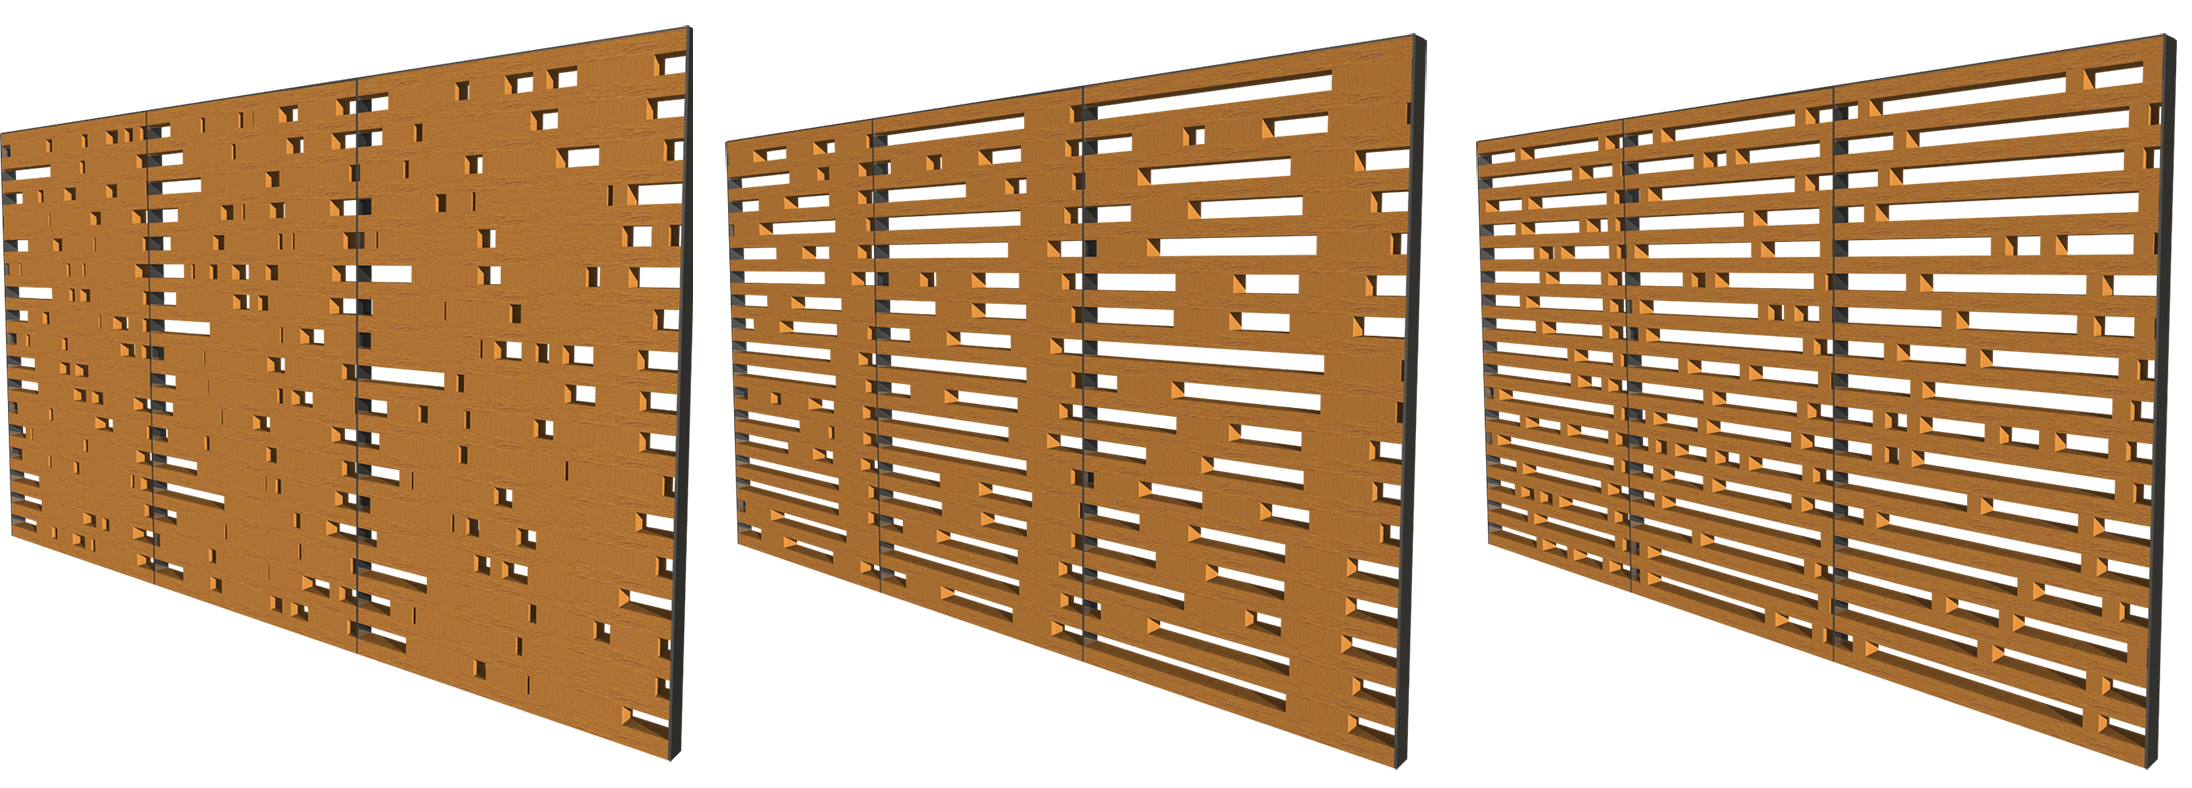
\includegraphics[width=\columnwidth]{../report/Images/Evaluation/ericeira_extended_abstract.png}
	\caption{Ericeira Solarium: Representation of the shading panels’ geometric pattern with different sUDI values (from left to right, 7\%, 90\%, and 100\%).}
	\label{fig:ericeira_multiple_panels}
\end{figure}

 We benchmarked the performance of $13$ different derivative-free optimization algorithms: $5$ direct-search, $3$ metaheuristics, and $5$ model-based. Given that each objective function evaluation takes $7$ minutes to complete, we set a limit of $60$ evaluations per run.

%http://papers.cumincad.org/data/works/att/caadria2018\_278.pdf
\begin{table}[]
	\centering
	\includegraphics[width=\columnwidth]{Images/ericeira/phase1_stats_EA.pdf}	
	\caption{Ericeira Solarium: Table with the mean best daylight results and mean evaluations to reach optimal solutions of each algorithm. Results are averaged over three runs, each with $60$ evaluations.}
	\label{table:phase1results}
\end{table}

\Cref{table:phase1results} shows the mean best results and the standard deviation of the three runs, discriminated by algorithm. According to the results, in average, the global model-based algorithms \textit{GPR}, \textit{RBFCC}, and \textit{RBFCL} were able to find an optimal solution within the first $30$ evaluations. Conversely, the local model-based algorithms \textit{\ac{COBYLA}} and \textit{\ac{BOBYQA}} performed rather poorly in this problem, converging to far from optimal solutions after $29$ and $48$ function evaluations, respectively. Regarding direct-search algorithms, the global algorithm \textit{\ac{DIRECT}} was able to find a close to optimal solution (with an \ac{sUDI} value of $98\%$) in the last function evaluation. Its local variant, \textit{\ac{DIRECT}-L}, and the local direct-search algorithms \textit{\ac{PRAXIS}} and \textit{SUBPLEX} fell short of the expected and barely managed to improve over $80\%$. Nevertheless, the simplex-based direct-search algorithm \textit{\ac{NMS}} performed surprisingly well, having achieved an average result of $89.67\%$ within the first $15$ evaluations. Finally, although metaheuristics performed better than most local model-based and direct-search algorithms, they seem to stagnate in design solutions with \ac{sUDI} values below the $88\%$, after $30$ evaluations.

\Cref{fig:phase1results} shows the average performance per algorithm class, also separating them in local or global algorithms. Overall, local algorithms seem to perform worse than all other algorithms, with local direct-search and model-based algorithms stagnating towards design solutions with \ac{sUDI} values below $75\%$ and $70\%$, respectively. Contrastingly, global algorithms were able to find design solutions with values of \ac{sUDI} larger than $80\%$. Despite the good initial performance of metaheuristics algorithms for the first $20$ evaluations, global direct-search algorithms quickly surpassed them, achieving close to optimal solutions with \ac{sUDI} values of $90\%$. Lastly, global model-based algorithms were, on average, the best performing algorithms, achieving close to optimal solutions shortly after $24$ evaluations. 

\begin{figure*}[]
	\centering
	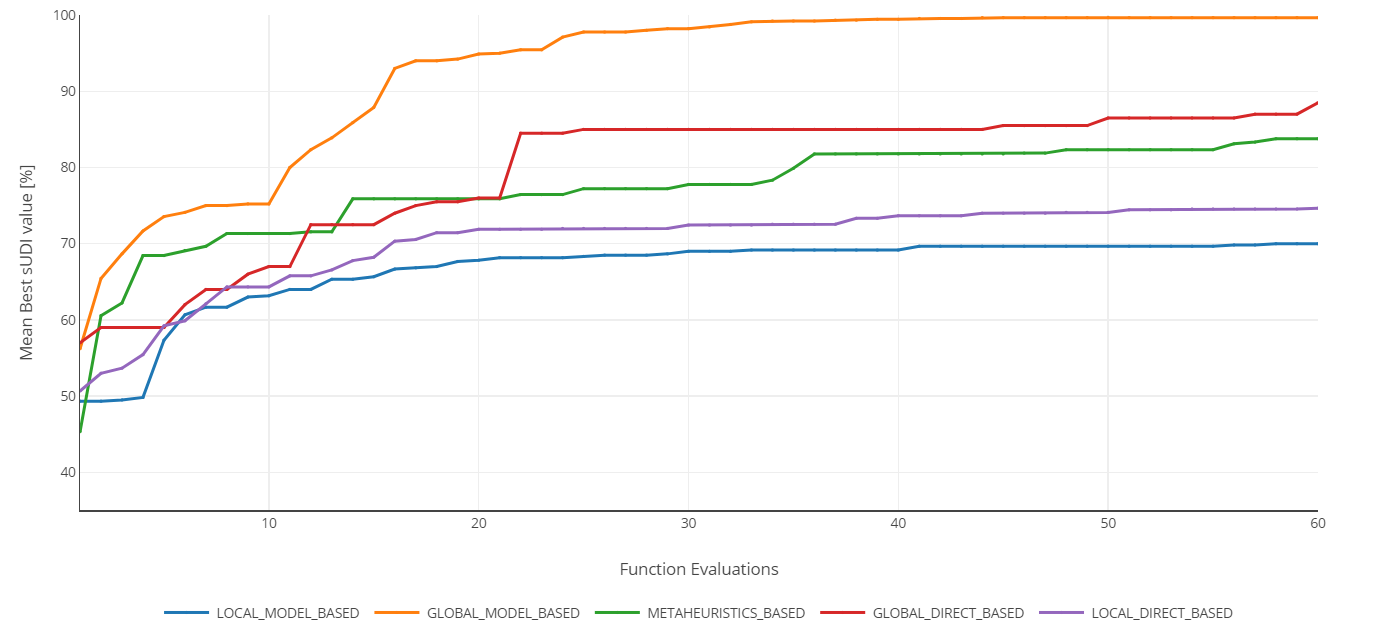
\includegraphics[width=2\columnwidth]{../report/Images/Evaluation/Ericeira_results_ph1_per_class.PNG}
	\caption{Ericeira Solarium: Mean best daylight results in function of the number of evaluations, discriminated per class of algorithms.}
	\label{fig:phase1results}
\end{figure*}

Given the overall bad performance of local algorithms, we decided to assess their performance when initialized with different solutions. Notwithstanding their ability to quickly converge to locally optimal solutions, the quality of the found solutions highly depends on the solution used to initialize the search. Therefore, we have also studied the impact of different initial solutions in the performance of these algorithms. To this end, we tested all $5$ local algorithms with two different initial solutions: a bad solution, with a $7\%$ value of \ac{sUDI}, and a reasonable solution with a $78\%$ value of \ac{sUDI}. Moreover, we decided to further restrict the number of evaluations to $15$, thus emulating an hypothetical scenario, where users lack knowledge about different optimization algorithms and opt for testing several of them. Ideally, this would allow them to infer the most promising algorithm and obtain a reasonable solution to hot-start other algorithms and, potentially, improve the overall optimization time. Results show that when provided with a mild solution, most local algorithms were able to converge to solutions with a $99\%$ value of \ac{sUDI} after $8$ evaluations (or $56$ minutes), against the $25$ evaluations (or approximately $3$ hours) required by global model-based algorithms. Conversely, as expected local algorithms performed poorly when provided with a bad initial solution, barely managing to improve over the initial value.

\subsection{Multi-Objective Optimization: Space Frame Optimization}
This case study consists in the \ac{MOO} of both the structural behavior and an \textit{ad-hoc} measure of the irregularity of an arc-shaped space frame. The irregularities are caused by three attractors that cause a deformation in the shape of the truss. To measure the goals for each design variant, we used the Robot analysis tool to compute the maximum displacement of the structure, and the sum of the Euclidean distances between the attractors. To increase the interest of this case study, we set out to minimize both objectives, thus promoting the conflict between them: placing the attractors near each other will weaken the structure and, thus, increase the maximum displacement of the space frame. In fact, to reduce the maximum displacement, the attractors should be scattered across the space frame but this implies larger distances among the three attractors, thus worsening the second objective. \Cref{fig:spaceframe} illustrates two examples of the space frame structure.
 
\begin{figure}[]
	\centering
	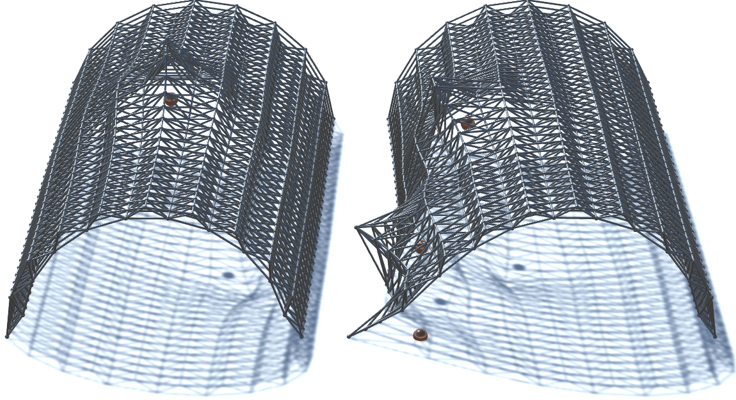
\includegraphics[width=\columnwidth]{Images/spaceframe/truss-kat-small.png}
	\caption{Space Frame: Representation of two design variations of the arc-shaped space frame, with copper balls representing the three attractors.}
	\label{fig:spaceframe}
\end{figure}

We benchmarked $10$ metaheuristics and $9$ model-based algorithms. On the one hand, each metaheuristic algorithm comprised a total of $15$ individuals/particles per iteration, which were evolved for $15$ iterations. On the other hand, model-based algorithms derived $100$ initial samples using the \textit{Latin Hypercube sampling} algorithm, which were then used to create the initial approximation to the expensive evaluation function, upon which another $125$ evaluations were completed. Overall, every algorithm was limited to a total of $225$ function evaluations, each taking approximately $40$ seconds to complete. In total, each run is composed of $4275$ candidate solutions and takes approximately $2$ days to complete.

Moreover, given the lack of more standardized approaches regarding the best way to evaluate the performance of \ac{MOO} algorithms, we evaluate them using a set of indicators measuring the cardinality, the diversity, and the accuracy of the results returned by each algorithm, i.e., the \acp{aPF}. \Cref{table:spaceframe} presents part of the obtained results averaged over the three runs, discriminated by the algorithms' classes and subclasses.

Although some indicators measure aspects based exclusively on the \acp{aPF}, others require a reference set to compare with the \acp{aPF}. Ideally, this reference set would represent the real optimal solutions for the specified problem. Unfortunately, this set of optimal solutions, also called \ac{tPF}, is not known for most \ac{BPO} problems. In an attempt to better approximate it, we compute a fictitious Pareto Front, the \ac{cPF}, composed of the best solutions found by each algorithm. 

Note, however, that we aimed at measuring the average performance of each algorithm regarding an unknown \ac{tPF}. In general, computing an accurate approximation of the \ac{tPF} would require running the algorithms for thousands of iterations, which is not feasible in most \ac{BPO} problems involving time-consuming evaluation functions. As a consequence, we adopted a methodology similar to the one used in the previous case study, which quantifies the performance of each algorithm in terms of the mean value of three runs, using as reference, for each run, the corresponding \acp{cPF}. 

\begin{table}[]
	\centering
	\label{table:spaceframe}
	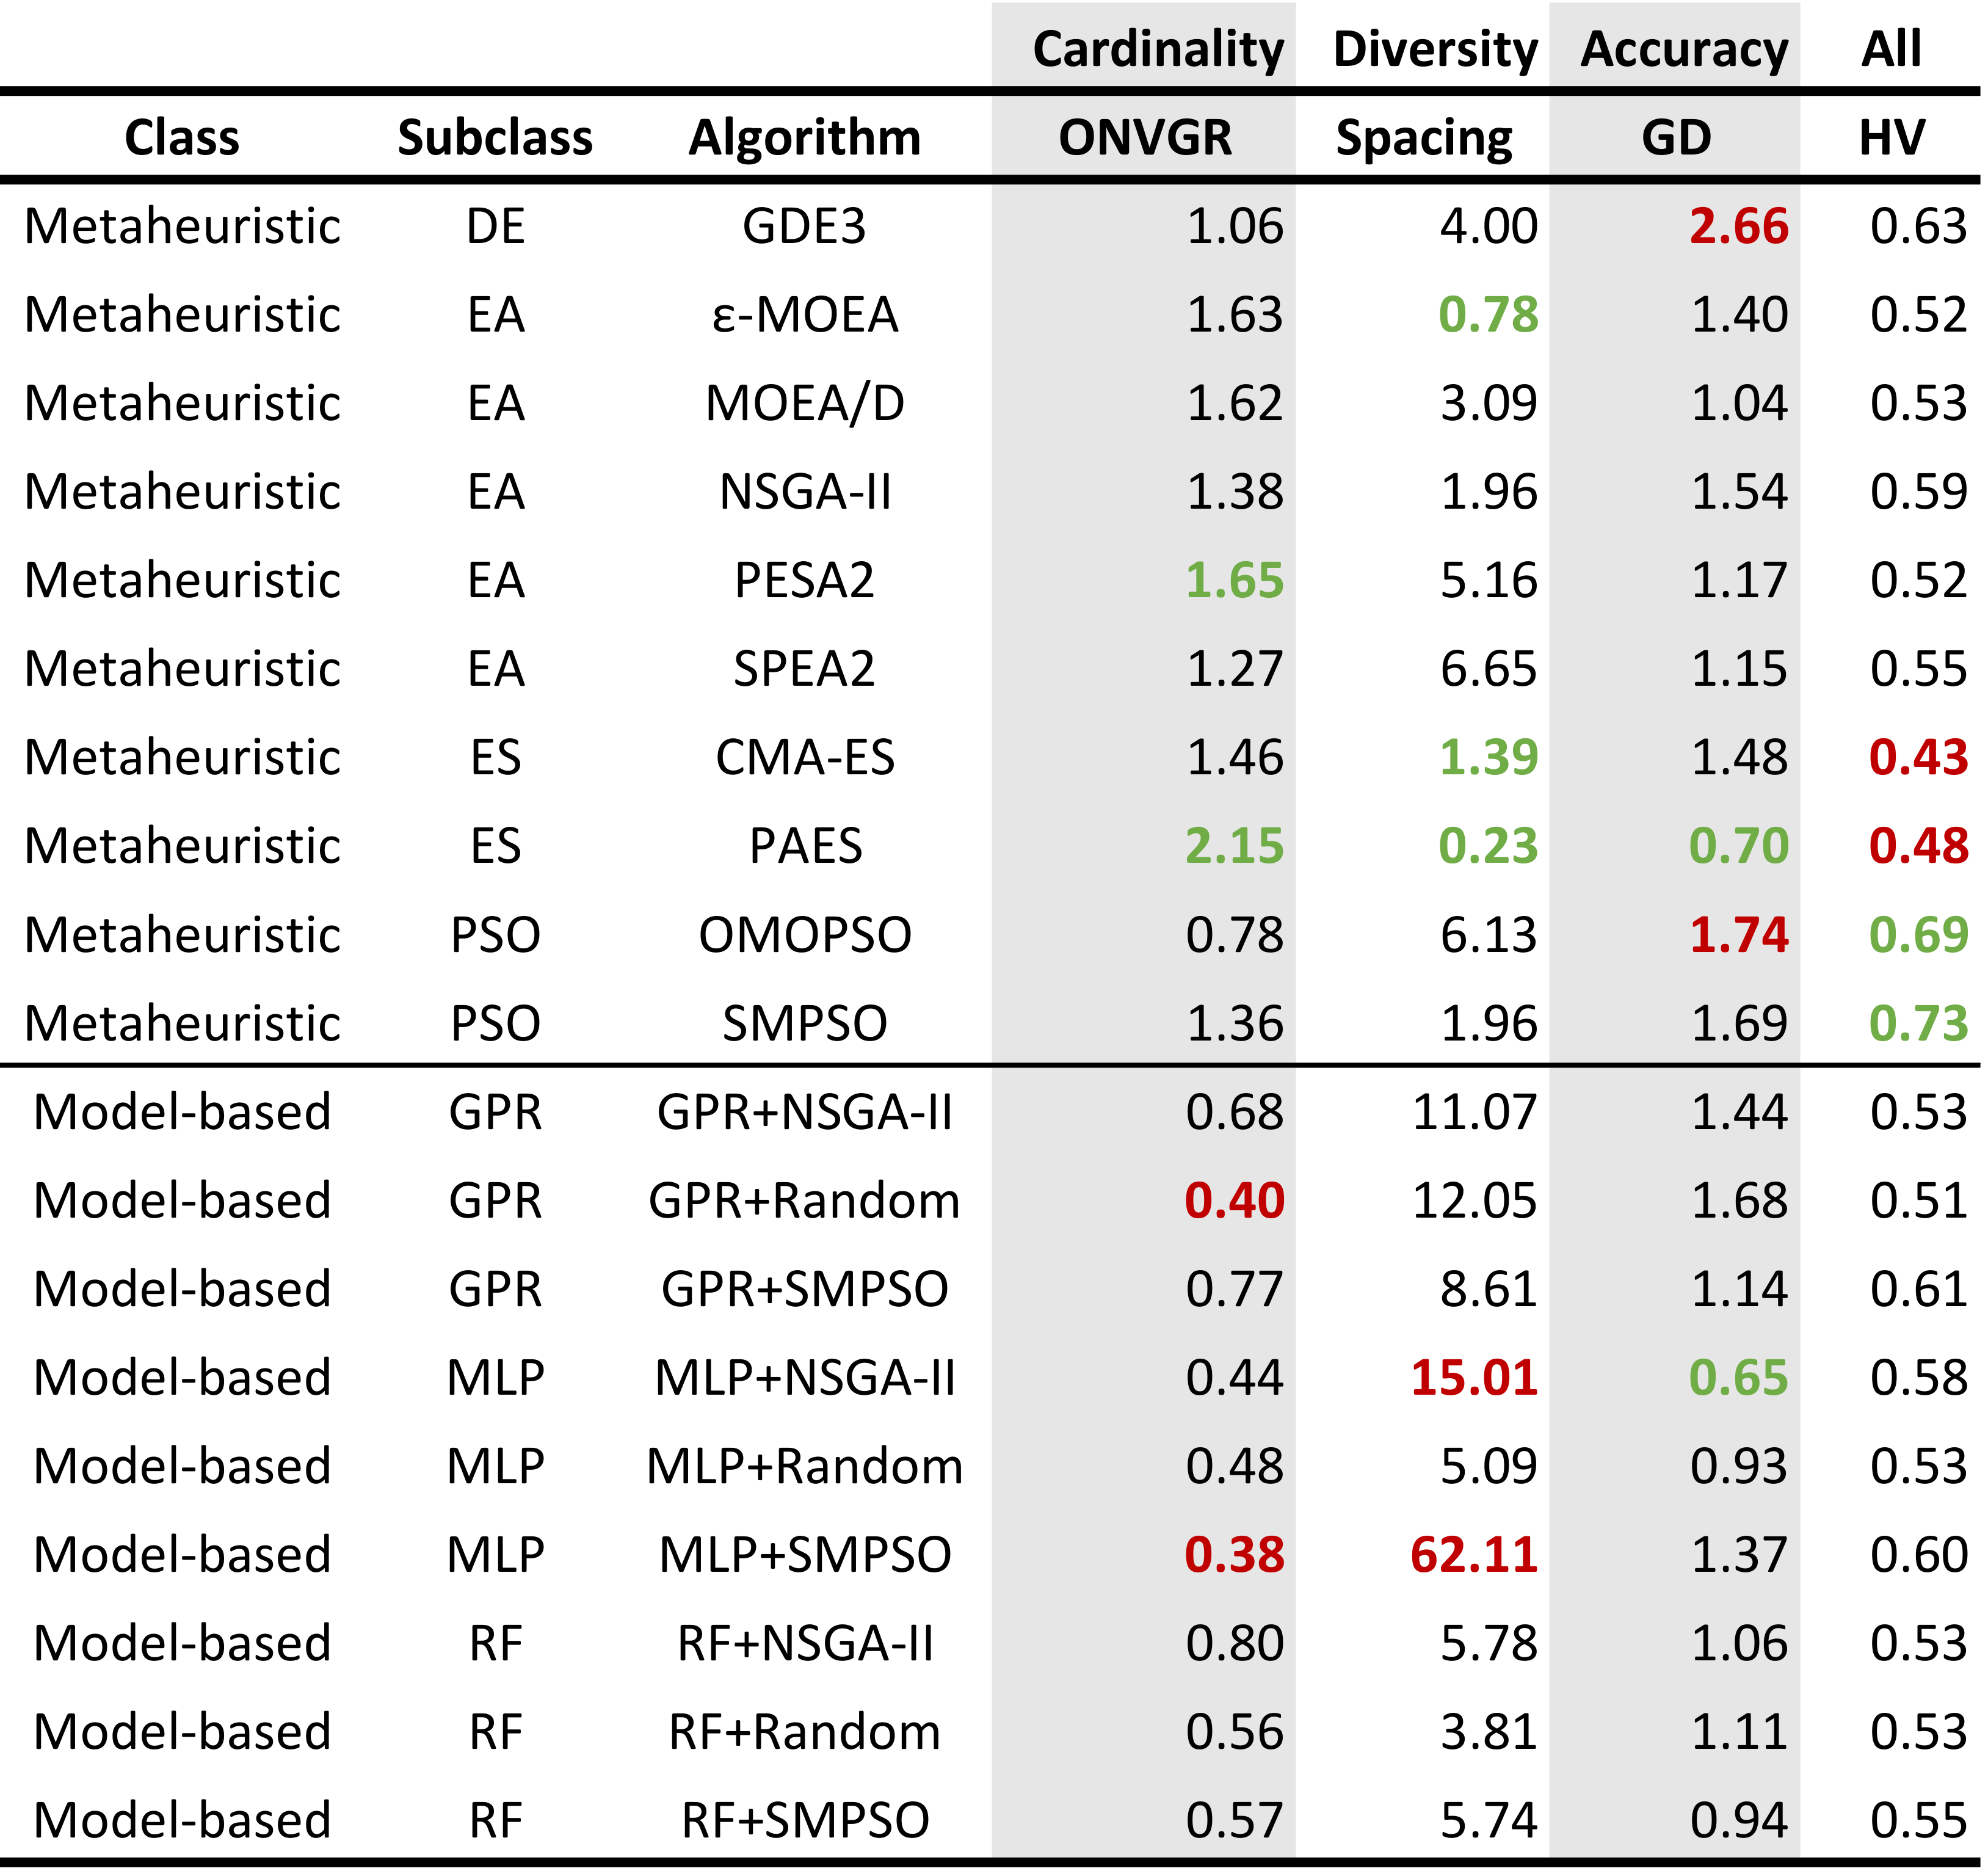
\includegraphics[width=\columnwidth]{Images/spaceframe/indicators_by_alg_mean_20190509.png}
	\caption{Space Frame: Mean values for the different aspects of the Pareto fronts, discriminated by algorithm. Results are averaged over $3$ runs, each with $225$ evaluations.}
\end{table}

To measure the cardinality aspect, we consider the \ac{ONVGR} indicator, which computes the ratio of optimal solutions between \acp{aPF} and \acp{cPF}. In general, metaheuristics seem to retrieve the most nondominated solutions within each run, whereas model-based algorithms seem to retrieve the least. In fact, among the model-based algorithms, the algorithms exploring random search strategies, i.e., the algorithms suffixed with \textit{Random}, yield fewer nondominated solutions, which may result from a poor exploration of the solution space. On average, the best performing algorithm, \textit{PAES}, is able to find twice the number of solutions that compose each \ac{cPF}, whereas model-based algorithms, including \textit{GPR+Random} and \acp{MLP} algorithms, struggled to find a set of optimal solutions with at least half of the size of the \acp{cPF}. While this indicator provides an intuition about the richness of each algorithm's \acp{aPF}, many of the identified solutions might not be truly optimal, i.e., despite being optimal among all the evaluated solutions, these solutions might not belong to the corresponding \ac{cPF}. To this end, other indicators should also be considered, such as \ac{ER}.

On the other hand, Spacing was used to measure the diversity of the \acp{aPF}, as it provides an estimate of the uniformity of the \acp{aPF}' distribution. Considering this indicator, the two \ac{ES} metaheuristic algorithms, \textit{PAES} and \textit{CMA-ES}, and one \ac{EA}-based metaheuristic algorithm, $\epsilon$\textit{-MOEA}, achieved the most uniform \acp{aPF}. Conversely, model-based algorithms seem to yield more irregular \acp{aPF}, namely, \textit{MLP+NSGA-II} and \textit{MLP+SMPSO} achieved the worst values of Spacing. Note, however, that this indicator merely provides an idea of the regularity of distribution of the solutions. Ideally, this indicator would also suggest a good coverage of the \ac{cPF}, i.e., that the \acp{aPF} found by each algorithm cover the same regions as the \acp{cPF}, instead of focusing on narrower regions. However, most of the algorithms that present the best Spacing scores achieve such values because most of the identified optimal solutions lie within the same small region but present a more uniform distribution. Besides this limitation, these indicators are also highly sensitive to outliers and to the number of retrieved solutions. Besides having an uniform distribution, it is also important to have a measure of the extent of each Pareto front (e.g., using the Maximum Spread indicator), as it implies that more relevant trade-offs are provided.

Another important aspect of \acp{aPF} is their accuracy and how close their solutions are from the \acp{cPF}. In this paper, we merely focus on the \ac{GD} indicator, which measures the average approximation of each algorithm's \acp{aPF} to the closest solutions in the corresponding \acp{cPF}. \Cref{table:spaceframe} shows that, on average, \textit{MLP+NSGA-II} and \textit{PAES} present the best convergence towards the \ac{cPF}, and that \textit{GDE3} and \textit{OMOPSO} present the worst convergence values. These can be explained by the number of the nondominated solutions retrieved by each algorithm, as well as by the creation of clusters of optimal solutions near the \acp{cPF} that were discovered by \textit{PAES} and \textit{MOEA/D}. In general, other model-based algorithms also present reasonable scores, like the \textit{MLP+Random} or all the \ac{RF}-based algorithms even surpassing many metaheuristics algorithms, including \textit{CMA-ES}, $\epsilon$\textit{-MOEA}, \textit{NSGA-II}, and \textit{SPEA2}, thus suggesting better approximations.

In the end, we also used the \ac{HV} indicator, as it appraises the quality of a Pareto front with regards to all three aspects simultaneously. The best performing algorithms were the \ac{PSO}-based algorithms, \textit{SMPSO} and \textit{OMOPSO}, followed by \textit{GDE3}. Surprisingly, the \ac{PSO} model-based algorithms also present a good performance, when compared to other metaheuristics, and even to other model-based algorithms that explore \textit{Random} or \ac{EA} strategies to search for optimal solutions. Conversely, the worst performing algorithms were the \ac{ES}-based ones, \textit{CMA-ES} and \textit{PAES}, followed by \textit{GPR+Random}. 

\begin{figure*}[hptb]
	\centering
	\includegraphics[width=2\columnwidth]{../report/Images/Evaluation/caadria/All_Algorithms_all_runs-2019-04-13_1000dpi.png}
	\caption[Space Frame: Pareto front plot]{Space Frame: Algorithms' \acp{aPF} measuring the attractors distance, in function of the maximum displacement. These fronts are obtained by combining the values of the $3$ runs for each algorithm. The \ac{cPF} is formed by finding the nondominated solutions from all the evaluated solutions.}
	\label{fig:allruns}
\end{figure*}

Overall, no single algorithm was able to outperform the others in terms of all the indicators. Nevertheless, the \ac{PSO}-based metaheuristics algorithms, \textit{OMOPSO} and \textit{SMPSO}, exhibited the overall best performance. Moreover, even though none of the model-based algorithms was able to surpass the \textit{SMPSO} and \textit{OMOPSO}, the model-based algorithms that use \textit{SMPSO} also exhibited a reasonable performance, better than several well-known metaheuristics, including $\epsilon$\textit{-MOEA}, \textit{MOEA/D}, \textit{CMA-ES}, and \textit{SPEA2}. \Cref{fig:allruns} presents a combined view of all the algorithms for every run, where it is possible to visualize the extent of \ac{PSO}-based algorithms and the high density region to which several \acp{EA} and \acp{ES} algorithms converged.
